\chapter{Mini-experiments}~\label{appendix-mini-experiments}

\section{Experiences with a test Android app: Travel Europe}
The author co-created a small functional test app, called \myindex{Travel Europe}, with Joe Reeve. It is available in Google Play for pre-release testing (it has not been published yet). The app incorporates Microsoft's App Center Analytics and content known as Travel Europe that was collated automatically by the Kiwix project and made freely available for use and re-use.

We created the Android test app, in Kotlin. Initially it had at least one known flaw (in release 6) that causes the app to crash with an unhandled exception. Several test releases were uploaded to the app store over several weeks.

We wanted to track whether Google Play Console detects the installation, activity, and any crashes that occur.

\subsection{From Zero to Ten}
For our test app we configured 10 additional valid Google accounts and invited each of these to be testers of the new as yet unreleased app. These accounts belong to a domain owned by one of the authors, otherwise they are standard Google accounts as far as we know. Each of these accounts was assigned to a different physical Android device.

There was a per account opt-in to be a tester for the app (using a convoluted process) before the app could be downloaded.\sidenote{This would not be necessary for apps available as a general release in Google Play.} Version 6 was installed and run on each of the devices. After the app had crashed on each of the devices the mobile analytics reports were checked.

An updated release of the app (release 7) was created that fixed the crash and it was uploaded to Google Play as another test release. This was installed and run on each of the devices.

\subsection{Pre-launch report automated testing}
For release 6 of the test app crashes were found on 10 of the 12 devices used by the automated monkey testing (which uses Google Android's Robo automated test tool on their Firebase Test Lab's physical devices). The test runs for the two crash-free devices did not happen to click on content that triggered the exception.

\subsection{Google Play Console and Android Vitals reporting}
Initially, Google Play Console and Android Vitals included usage and errors for the app. These mysteriously stopped a few days later and none of the ramp up to 10+ users has been recorded. As activity is shown for most days for most of the apps the authors have access to, it is not clear whether the omission is by design, accident, or a glitch in the processing system.

\subsection{Microsoft App Center reporting}
Microsoft's App Center\index{Microsoft App Center} Analytics seems to track activity within a minute of it occurring. It records one active user in the United States, seven in the United Kingdom and 21 Unknown. Some of the 'users' may be those in Firebase Test Lab (used by Google for the automated pre-launch testing), however we have yet to determine the causes for the 21 unknown locations (the app does not explicitly ask for location permissions on behalf of the \myindex{Microsoft App Center} library incorporated in the app). It also counted one device (a HTC Desire 510) twice, perhaps as it had both debug developer builds and the app from the app store installed at different times?

App Center limits various details to the top 4 items, for instance the "Top devices" and "OS Distribution", the lack of detail is unhelpful. In contrast Google Play Console sometimes provides many more items, the exact amount depends on several factors the author is still investigating.

\begin{figure}
    \centering
    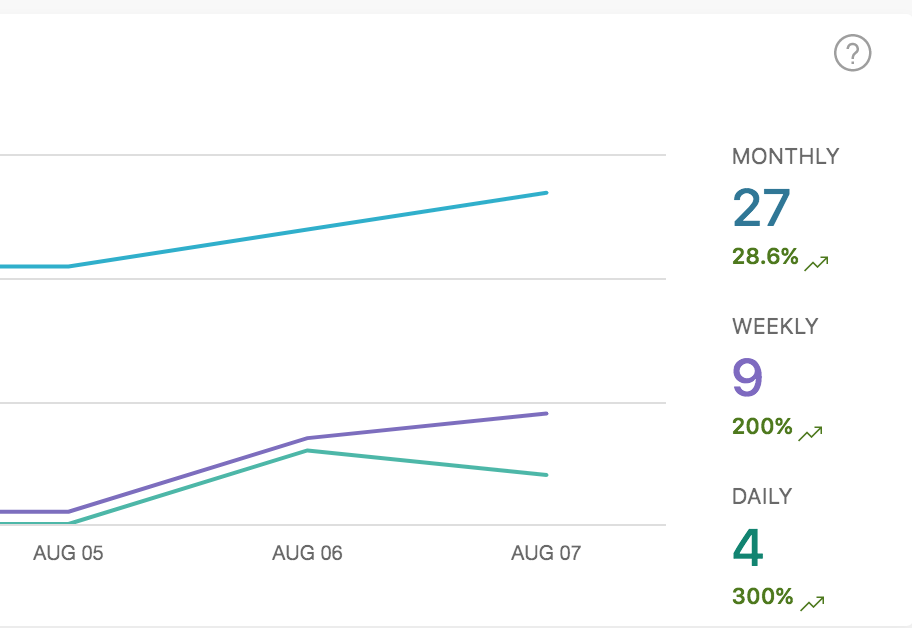
\includegraphics[width=\linewidth]{images/microsoft-app-center/AppCenter_snippet_growth_for_test_app_2019_Aug_07.png}
    \caption{Microsoft App Center user growth for Travel Europe}
    \label{fig:appcenter_user_growth}
\end{figure}

\begin{figure*}[htbp]
    \centering
    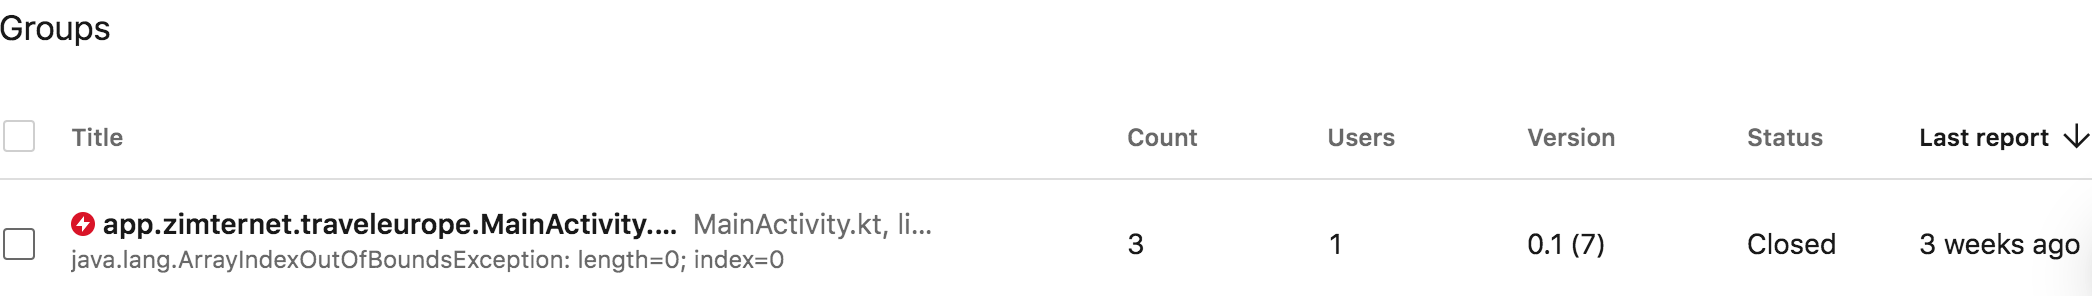
\includegraphics[width=\linewidth]{images/microsoft-app-center/AppCenter_crash_reported_in_test_app_2019_aug_07.png}
    \caption{Microsoft App Center crash reported for the Travel Europe app}
    \label{fig:appcenter_crash_report}
\end{figure*}

Microsoft App Center did not detect crashes that happened in August 2019, the last instance they detected was 3 weeks earlier in July 2019, see Figure \ref{fig:appcenter_crash_report}.

\subsection{Conclusions}
This mini-experiment provided insights into using in-app analytics during pre-release stages of app development, where some usage was recorded by Microsoft App Center. Disturbingly some of the crashes were not reported in either \myindex{Microsoft App Center} or Google Play Console with \myindex{Android Vitals}. Had none of the crashes appeared in Google Play Console then one option was they do not report on pre-release apps, however the existence of some crashes indicates this hypothesis is incorrect.